\section{FESDModelv2 Results}

The results of the testing after 100 epochs of training for FESDModelv2 can be seen in table \ref{tab:res_v2}. The numeric values of the accuracy and F1-Score show good results. However, the percentage of positive guesses metric seems to hint at overfitting.

\begin{table}
  \caption[Test Results of FESDModelv2]{The test results of FESDModelv2 after 100 epochs of training.}
  \label{tab:res_v2}
  \centering
  \begin{tabular}{p{0.15\linewidth}p{0.15\linewidth}p{0.15\linewidth}p{0.15\linewidth}p{0.15\linewidth}}
    \hline
    {} &  Percentage of positive guesses &  Accuracy &  F1-Score &  Cohen's Kappa Coefficient \\
    Problem Set   &                                 &           &           &                            \\
    \hline
    Full Body  &                         100.000 &     0.725 &     0.725 &                      0.000 \\
    Half Body  &                          78.542 &     0.698 &     0.525 &                      0.370 \\
    Body Parts &                         100.000 &     0.874 &     0.874 &                      0.000 \\
    Joints     &                          70.010 &     0.892 &     0.638 &                      0.772 \\
    \hline
  \end{tabular}
\end{table}

The results shown in table \ref{tab:res_v2} are reflected in the confusion matrices seen in figure \ref{fig:conf_v2}. The half-body and body parts problem set only guess positive results, hence the Percentage of positive guesses. The Cohen's Kappa Coefficient is 0 if $tp \cdot tn = fn \cdot fp$. This is the case if only one class is guessed, which is the case if all guesses are positive.

\begin{figure}
  \centering
  \begin{subfigure}[b]{0.47\linewidth}
      \centering
      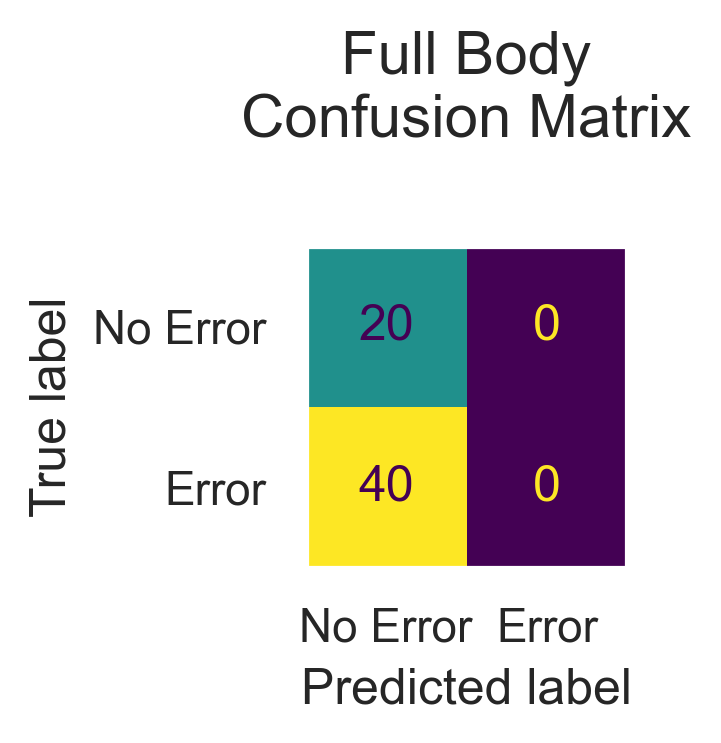
\includegraphics[width=\textwidth]{figures/Results/v2/confusion/full_together.png}
      \caption[]{Full Body Problem Set}
      \label{fig:fb_conf}
  \end{subfigure}
  \hfill
  \begin{subfigure}[b]{0.47\linewidth}
      \centering
      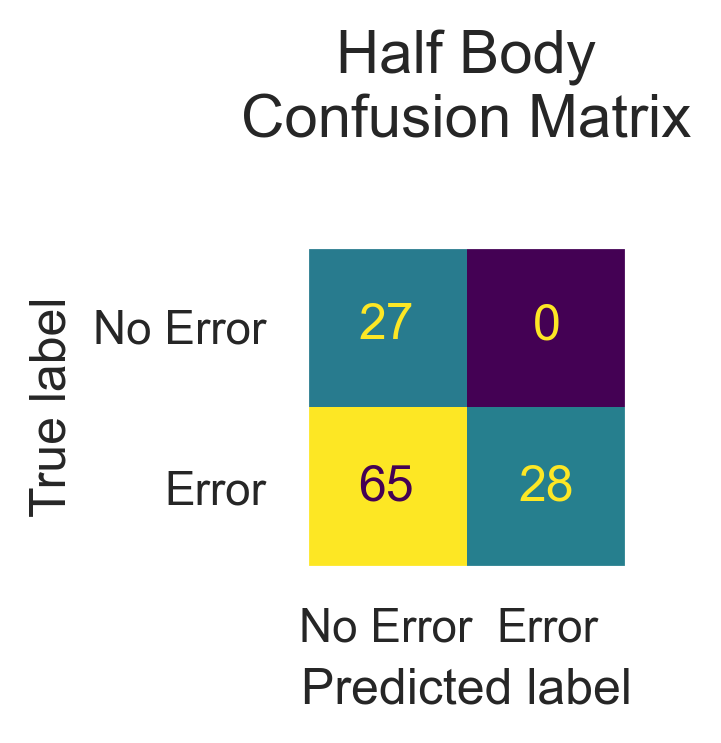
\includegraphics[width=\textwidth]{figures/Results/v2/confusion/half_together.png}
      \caption{Half Body Problem Set}
      \label{fig:hb_conf}
  \end{subfigure}
  \hfill
  \begin{subfigure}[b]{0.47\linewidth}
      \centering
      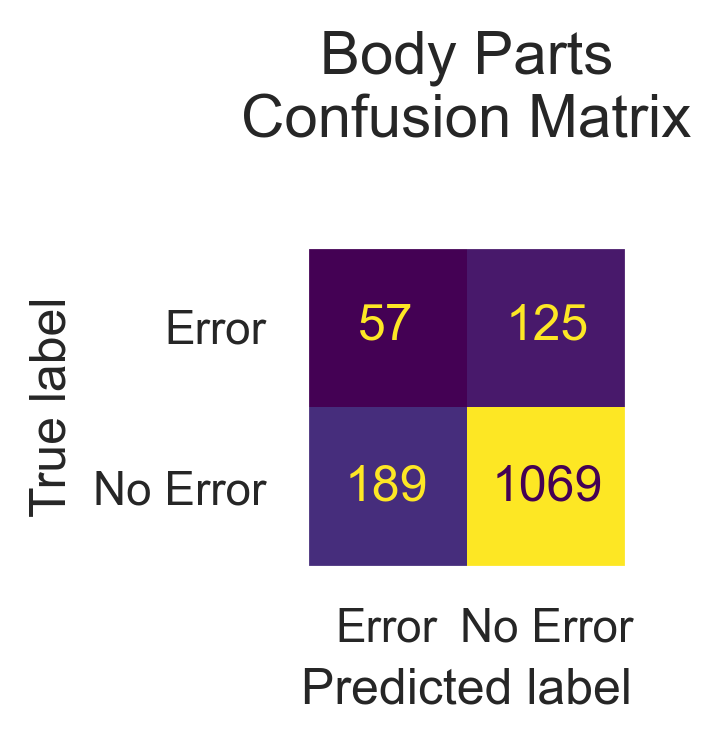
\includegraphics[width=\textwidth]{figures/Results/v2/confusion/body_parts_together.png}
      \caption{Body Part Problem Set}
      \label{fig:bp_conf}
  \end{subfigure}
  \hfill
  \begin{subfigure}[b]{0.47\linewidth}
      \centering
      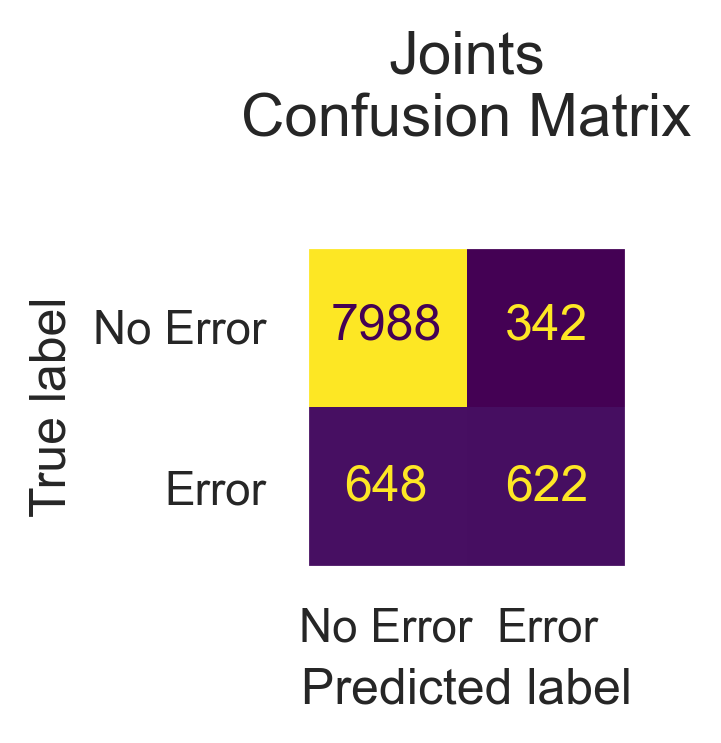
\includegraphics[width=\textwidth]{figures/Results/v2/confusion/joints_together.png}
      \caption{Joint Problem Set}
      \label{fig:jt_conf}
  \end{subfigure}
  \caption[Confusion Matrices of FESDModelv2]{The confusion Matrices of FESDModelv2.}
  \label{fig:conf_v2}
\end{figure}

While the half-body and joint models seem to achieve good results, the ROC-curve shown in figure \ref{fig:roc_v2}, shows that also these models perform badly.

\begin{figure}
  \centering
  \begin{subfigure}[b]{0.47\linewidth}
      \centering
      \includegraphics[width=\textwidth]{figures/Results/v2/fb/roc.png}
      \caption[]{Full Body Problem Set}
      \label{fig:fb_roc_v2}
  \end{subfigure}
  \hfill
  \begin{subfigure}[b]{0.47\linewidth}
      \centering
      \includegraphics[width=\textwidth]{figures/Results/v2/hb/roc.png}
      \caption[]{Half Body Problem Set}
      \label{fig:hb_roc_v2}
  \end{subfigure}
  \hfill
  \begin{subfigure}[b]{0.47\linewidth}
      \centering
      \includegraphics[width=\textwidth]{figures/Results/v2/bp/roc.png}
      \caption[]{Body Part Problem Set}
      \label{fig:bp_roc_v2}
  \end{subfigure}
  \hfill
  \begin{subfigure}[b]{0.47\linewidth}
      \centering
      \includegraphics[width=\textwidth]{figures/Results/v2/jt/roc.png}
      \caption[]{Joint Problem Set}
      \label{fig:jt_roc_v2}
  \end{subfigure}
  \caption[ROC Curves of FESDModelv2]{The ROC curves of FESDModelv2.}
  \label{fig:roc_v2}
\end{figure}

The ROC curve shows that also the model for the half-body and joint problem set is no better than a random classifier due to over-confidence regardless of the result.